\PassOptionsToPackage{unicode=true}{hyperref} % options for packages loaded elsewhere
\PassOptionsToPackage{hyphens}{url}
\documentclass[11pt,dvipsnames,ignorenonframetext,aspectratio=169]{beamer}
\IfFileExists{pgfpages.sty}{\usepackage{pgfpages}}{}
\setbeamertemplate{caption}[numbered]
\setbeamertemplate{caption label separator}{: }
\setbeamercolor{caption name}{fg=normal text.fg}
\beamertemplatenavigationsymbolsempty
\usepackage{lmodern}
\usepackage{amssymb,amsmath}
\usepackage{ifxetex,ifluatex}
\usepackage{fixltx2e} % provides \textsubscript
\ifnum 0\ifxetex 1\fi\ifluatex 1\fi=0 % if pdftex
  \usepackage[T1]{fontenc}
  \usepackage[utf8]{inputenc}
\else % if luatex or xelatex
  \ifxetex
    \usepackage{mathspec}
  \else
    \usepackage{fontspec}
\fi
\defaultfontfeatures{Ligatures=TeX,Scale=MatchLowercase}







\fi

  \usetheme[]{monash}

  \usecolortheme{monashwhite}


% A default size of 24 is set in beamerthememonash.sty


  \useinnertheme{rounded}

  \useoutertheme{smoothtree}

% use upquote if available, for straight quotes in verbatim environments
\IfFileExists{upquote.sty}{\usepackage{upquote}}{}
% use microtype if available
\IfFileExists{microtype.sty}{%
  \usepackage{microtype}
  \UseMicrotypeSet[protrusion]{basicmath} % disable protrusion for tt fonts
}{}


\newif\ifbibliography


\hypersetup{
      pdftitle={Population genetics},
            colorlinks=true,
    linkcolor=red,
    citecolor=Blue,
    urlcolor=lightgrayd,
    breaklinks=true}
%\urlstyle{same}  % Use monospace font for urls







% Prevent slide breaks in the middle of a paragraph:
\widowpenalties 1 10000
\raggedbottom

  \AtBeginPart{
    \let\insertpartnumber\relax
    \let\partname\relax
    \frame{\partpage}
  }
  \AtBeginSection{
    \ifbibliography
    \else
      \let\insertsectionnumber\relax
      \let\sectionname\relax
      \frame{\sectionpage}
    \fi
  }
  \AtBeginSubsection{
    \let\insertsubsectionnumber\relax
    \let\subsectionname\relax
    \frame{\subsectionpage}
  }



\setlength{\parindent}{0pt}
\setlength{\parskip}{6pt plus 2pt minus 1pt}
\setlength{\emergencystretch}{3em}  % prevent overfull lines
\providecommand{\tightlist}{%
  \setlength{\itemsep}{0pt}\setlength{\parskip}{0pt}}

  \setcounter{secnumdepth}{0}


%% Monash overrides
\AtBeginSection[]{
   \frame<beamer>{
   \frametitle{Outline}\vspace*{0.2cm}
   
   \tableofcontents[currentsection,hideallsubsections]
  }}

% Redefine shaded environment if it exists (to ensure text is black)
\ifcsname Shaded\endcsname
  \definecolor{shadecolor}{RGB}{225,225,225}
  \renewenvironment{Shaded}{\color{black}\begin{snugshade}\color{black}}{\end{snugshade}}
\fi
%%

  \usepackage{setspace}
  \usepackage{wasysym}
  % \usepackage{footnote} % don't use this this breaks all
  \usepackage{fontenc}
  \usepackage{fontawesome}
  \usepackage{booktabs,siunitx}
  \usepackage{longtable}
  \usepackage{array}
  \usepackage{multirow}
  \usepackage{wrapfig}
  \usepackage{float}
  \usepackage{colortbl}
  \usepackage{pdflscape}
  \usepackage{tabu}
  \usepackage{threeparttable}
  \usepackage{threeparttablex}
  \usepackage[normalem]{ulem}
  \usepackage{makecell}
  \usepackage{xcolor}
  \usepackage{tikz} % required for image opacity change
  \usepackage[absolute,overlay]{textpos} % for text formatting
  \usepackage{chemfig}
  \usepackage[skip=0.333\baselineskip]{caption}
  % \newcommand*{\AlignChar}[1]{\makebox[1ex][c]{\ensuremath{\scriptstyle#1}}}%
  
  % this font option is amenable for beamer
  \setbeamerfont{caption}{size=\tiny}
  \singlespacing
  \definecolor{lightgrayd}{gray}{0.95}
  \definecolor{skyblued}{rgb}{0.65, 0.6, 0.94}
  \definecolor{oranged}{RGB}{245, 145, 200}

  \title[]{Population genetics}


  \author[
        Deependra Dhakal\\
Gokuleshwor Agriculture and Animal Science College\\
Tribhuwan University\\
\textit{ddhakal.rookie@gmail.com}\\
\url{https://rookie.rbind.io}
    ]{Deependra Dhakal\\
Gokuleshwor Agriculture and Animal Science College\\
Tribhuwan University\\
\textit{ddhakal.rookie@gmail.com}\\
\url{https://rookie.rbind.io}}


\date[
      Academic year 2019-2020
  ]{
      Academic year 2019-2020
        }

\begin{document}

% Hide progress bar and footline on titlepage
  \begin{frame}[plain]
  \titlepage
  \end{frame}


   \frame<beamer>{
   \frametitle{Outline}\vspace*{0.2cm}
   
   \tableofcontents[hideallsubsections]
  }

\hypertarget{gene-and-genotypes}{%
\section{Gene and genotypes}\label{gene-and-genotypes}}

\begin{frame}{What is allele/gene ?}
\protect\hypertarget{what-is-allelegene}{}

An allele/gene is the bit of DNA at the place called locus (the place on
a chromosome where an allele resides). An allele is instantiation of a
locus. But by orthology, a locus is not template for an allele.
Similarly, a locus is not tangible, rather a map describing where to
find a tangible thing, an allele on a chromosome. A diploid individual
has two alleles at a particular autosomal locus.

\end{frame}

\begin{frame}{Genotype and allele frequencies}
\protect\hypertarget{genotype-and-allele-frequencies}{}

In A loci, suppose, two alleles \(A_1\) and \(A_2\) are present in a
diploid organism the genotype and genotypic frequency of segregating
population will be;

\[
\begin{aligned}
\textrm{Genotype} \hspace{20pt} & A_1A_1 & A_1A_2 \hspace{20pt} & A_2A_2 \\
\textrm{Relative frequency} \hspace{20pt} & x_{11} & x_{12} \hspace{20pt} & x_{22}
\end{aligned}
\]

As, relative frequencies must add to 1,

\[
x_{11} + x_{12} + x_{22} = 1
\]

The order of subscripting heterozygous is arbitrary.

Frequency of \(A_1\) allele in the population is,

\[
p = x_{11} + \frac{1}{2}x_{12}
\]

\end{frame}

\begin{frame}{}
\protect\hypertarget{section}{}

and frequency of \(A_2\) allele is,

\[
q = 1-p = x_{22} + \frac{1}{2}x_{12}
\]

Measure of each allele frequency can be thought of as independent
events. For e.g., for allele \(p\) to be selected;

\[
p = \left(x_{11} \times \frac{1}{P(p_{A_1A_1})}\right) + \left(x_{12} \times \frac{1}{2}\right) + (x_{22} \times 0)
\]

Where, \(P(p, A_1A_1)\) is the probability of getting \(p\) allele from
\(A_1A_1\) genotype, for loci with more than two alleles, frequency of
\(i^{th}\) allele will be called \(p_i\). Frequency of \(A_iA_j\)
genotype will be called \(x_ij\) for heterozygotes, \(i\neq j\) and, by
convention, \(i<j\).

\end{frame}

\begin{frame}{}
\protect\hypertarget{section-1}{}

If there are \(n\) alleles,

\[
\begin{aligned}
1 &= x_{11} + x_{22} + x_{33} + ... + x_{nn} + x_{12} + x_{13} + x_{(n-1)n} \\
  &= \sum^n_{i=1}\sum^n_{j\geq i}{x_{ij}}
\end{aligned}
\]

The frequency of \(i^th\) allele is

\[
p_i = x_{ii} + \frac{1}{2}\sum^{i-1}_{j = 1}{x_{ji}} + \frac{1}{2}\sum^n_{j = i+1}{x_{ij}}
\]

\end{frame}

\hypertarget{hardy-weinberg-law}{%
\section{Hardy-Weinberg law}\label{hardy-weinberg-law}}

\begin{frame}{}
\protect\hypertarget{section-2}{}

\begin{itemize}
\tightlist
\item
  In a random mating population (in which each male gamete has an equal
  chance of mating with any female gamete), when taken a loci with
  differences in alleles (A/a), following genotypes are possible:
  \(AA\), \(Aa\) and \(aa\).
\item
  With the corresponding frequencies of \(p^2\), \(2pq\) and \(q^2\),
  respectively for each of the genotypes, and bearing that gene
  frequencies must add up to unity, \(p^2+2pq+q^2 = 1\). This
  mathematical relationship is called the \textbf{Hardy-Weinberg
  equilibrium}.
\item
  Two scientists showed that the frequency of genotypes in a population
  depends on the frequency of genes in the preceding generation, not on
  the frequency of the genotypes.
\end{itemize}

\end{frame}

\begin{frame}{}
\protect\hypertarget{section-3}{}

\begin{itemize}
\tightlist
\item
  In each subsequent generation following thereafter, however, gene and
  genotypic frequencies will remain unchanged, provided that:

  \begin{enumerate}
  \tightlist
  \item
    Random mating occurs in a very large diploid population;
  \item
    Allele A and allele a are equally fit (one does not confer a
    superior trait than the other);
  \item
    There is no differential migration of one allele into or out of the
    population;
  \item
    The mutation rate of allele A is equal to that of allele a.
  \end{enumerate}
\end{itemize}

\end{frame}

\begin{frame}{Conservation of gene frequencies}
\protect\hypertarget{conservation-of-gene-frequencies}{}

\small

\begin{itemize}
\tightlist
\item
  Let us presume that among humans, the difference between those who can
  and those who cannot taste the chemical phenyl-thiocarbamate (PTC)
  resides in a single gene difference with two alleles, \(T\) and \(t\).
\item
  The allele for tasting, \(T\), is dominant over \(t\), so that
  heterozygotes, \(Tt\) are tasters, and the only nontasters are \(tt\).
\item
  If we were to choose an initial population composed of an arbitary
  number of each genotype, we may ask what will be the frequency of
  these genes after many generations.
\item
  Let us, for example, place upon an island a group of children in the
  ratio \(.40TT:.40Tt:.20tt\). The gene frequencies in this newly formed
  population are therefore, \(.4 + .2 = .6 T\), and \(.2 + .2 = .4t\).
\item
  Let us also assume that the number of individuals in the population is
  large, and the tasting or nontasting has no effect upon survival
  (viability), fertility, or attraction between the sexes.
\end{itemize}

\end{frame}

\begin{frame}{}
\protect\hypertarget{section-4}{}

\begin{itemize}
\tightlist
\item
  As these children mature, they will choose their mates at random from
  those of the opposite sex regardless of their tasting abilities.
\item
  Matings between any two genotypes can then be predicted solely on the
  basis of the frequency of those genotypes in the population.
\item
  Table \ref{tab:random-mating-monogene-gene-freq} shows matings in all
  possible combination.
\end{itemize}

\begin{table}[t]

\caption{\label{tab:random-mating-monogene-gene-freq}Types of random-mating combinations and their relative frequencies in a population containing .40TT, .40Tt, and .20tt genotypes}
\centering
\begin{tabular}{lrrr}
\toprule
gametes & TT & Tt & tt\\
\midrule
TT & 0.16 & 0.16 & 0.08\\
Tt & 0.16 & 0.16 & 0.08\\
tt & 0.08 & 0.08 & 0.04\\
\bottomrule
\end{tabular}
\end{table}

\end{frame}

\begin{frame}{}
\protect\hypertarget{section-5}{}

\begin{table}[t]

\caption{\label{tab:unnamed-chunk-1}Relative frequencies of the different kinds of offspring produced by the matings}
\centering
\begin{tabular}{lrlll}
\toprule
\multicolumn{2}{c}{Parents} & \multicolumn{3}{c}{Offspring ratio} \\
\cmidrule(l{3pt}r{3pt}){1-2} \cmidrule(l{3pt}r{3pt}){3-5}
Type of mating & Frequency of mating & TT & Tt & tt\\
\midrule
\rowcolor{gray!6}  $TT \times TT$ & 0.16 & all(.16) &  & \\
$TT \times Tt$ & 0.32 & 1/2(.32) & +1/2(.32) & \\
\rowcolor{gray!6}  $TT \times tt$ & 0.16 &  & all (.16) & \\
$Tt \times Tt$ & 0.16 & 1/4(.16) & +1/2 (.16) & +1/4(.16)\\
\rowcolor{gray!6}  $Tt \times tt$ & 0.16 &  & 1/2(.16) & +1/2(.16)\\
\addlinespace
$tt \times tt$ & 0.04 &  &  & all (.04)\\
\bottomrule
\end{tabular}
\end{table}

\end{frame}

\begin{frame}{}
\protect\hypertarget{section-6}{}

\begin{itemize}
\tightlist
\item
  Note that although the frequencies of genotypes have been altered by
  random mating, the gene frequencies have not changed.
\item
  For the \(T\) gene frequency is equal to \(.36 + 1/2(.48) = .60\), and
  the frequency of \(t\) is \(.16 + 1/2(.48) = .40\).
\item
  No matter what the initial frequencies of the three genotypes, the
  gene frequencies of the next generation will be the same as those of
  parental generation.
\end{itemize}

\end{frame}

\begin{frame}{Assertion}
\protect\hypertarget{assertion}{}

\begin{enumerate}
\tightlist
\item
  Under conditions of random mating ( \emph{panmixis}) in a large
  population where all genotypes are equally viable, gene frequencies of
  a particular generation depend upon the gene frequencies of the
  previous generation and not upon the \emph{genotype frequencies}.
\item
  The frequencies of different genotypes produced through random mating
  depend only upon the gene frequencies.
\end{enumerate}

\begin{itemize}
\tightlist
\item
  After the first generation of random mating, genotype frequencies also
  remain stable. i.e., equilibrium.
\end{itemize}

\end{frame}

\begin{frame}{Formal proof}
\protect\hypertarget{formal-proof}{}

\begin{table}[t]

\caption{\label{tab:unnamed-chunk-2}Mating combinations and frequencies of offspring produced under conditions of random mating when genotypic frequencies are $p^2TT$, $2pqTt$, and $q^2tt$}
\centering
\fontsize{6}{8}\selectfont
\begin{tabular}{>{\raggedright\arraybackslash}p{6em}>{\raggedright\arraybackslash}p{12em}>{\raggedright\arraybackslash}p{8em}>{\raggedright\arraybackslash}p{8em}>{\raggedright\arraybackslash}p{8em}}
\toprule
\multicolumn{2}{c}{Parents} & \multicolumn{3}{c}{Offspring ratio} \\
\cmidrule(l{3pt}r{3pt}){1-2} \cmidrule(l{3pt}r{3pt}){3-5}
Type of mating & Frequency of mating & TT & Tt & tt\\
\midrule
\rowcolor{gray!6}  $TT \times TT$ & $p^2 \times p^2 = p^4$ & $p^4$ &  & \\
$TT \times Tt$ & $2 \times p^2 \times 2pq = 4p^3q$ & $2p^3q$ & $2p^3q$ & \\
\rowcolor{gray!6}  $TT \times tt$ & $2 \times p^2 \times q^2 = 2p^2q^2$ &  & $2p^2q^2$ & \\
$Tt \times Tt$ & $2pq \times 2pq = 4p^2q^2$ & $p^2q^2$ & $2p^2q^2$ & $p^2q^2$\\
\rowcolor{gray!6}  $Tt \times tt$ & $2 \times 2pq \times q^2 = 4pq^3$ &  & $2pq^3$ & $2pq^3$\\
\addlinespace
$tt \times tt$ & $q^2 \times q^2 = q^4$ &  &  & $q^4$\\
\hline
\rowcolor{gray!6}   & $p^2(p^2 + 2pq + q^2) + 2pq(p^2 + 2pq + q^2) + q^2(p^2 + 2pq + q^2) = p^2 + 2pq + q^2 = (p + q)^2 = 1$ & $p^4 + 2p^3q + p^2q^2 = p^2(p^2 + 2pq + q^2) = p^2$ & $2p^3q + 4p^2q^2 + 2pq^3 = 2pq(p^2 + 2pq + q^2) = 2pq$ & $p^2q^2 + 2pq^3 + q^4 = q^2(p^2 + 2pq + q^2) = q^2$\\
\bottomrule
\end{tabular}
\end{table}

\end{frame}

\begin{frame}{Problem}
\protect\hypertarget{problem}{}

\begin{enumerate}
\setcounter{enumi}{2}
\tightlist
\item
  A population is consisted of 200 plants. Out of them, 100 plants are
  of Aa, 50 plants are of AA and 50 plants are of aa genotypes. This is
  a random mating population and in this population the frequencies of
  these three genotypes are at H-W equilibrium state. After \(5^{th}\)
  generations of random mating, plants having genotypes AA, Aa and aa
  are found in 500, 300 and 200 numbers respectively. Are they still in
  H-W equilibrium? Test the result with the help of \(\chi^2\) goodness
  of fit test.
\end{enumerate}

\end{frame}

\begin{frame}{Solution}
\protect\hypertarget{solution}{}

\begin{enumerate}
\setcounter{enumi}{2}
\tightlist
\item
  Here, the population of 200 plants is stated to be in H-W equilibrium;
  we already have equilibrium frequencies. Hence a \(\chi^2\) test for
  would show whether or not both the populations are same or have
  diverged from H-W equilibrium state (i.e.~observed frequncy of
  population after 5th generation is same or different than expected
  population frequency at initial condition). For facilitating
  comparison, we convert the given frequencies of observed genotypes
  (that of \(5^{th}\) generation) to the add upto current population
  count (200 individual).
\end{enumerate}

\end{frame}

\begin{frame}{}
\protect\hypertarget{section-7}{}

Thus observed frequencies are AA: 100; Aa: 60 and aa: 40.

Note, however, we commonly compute the expected frequency based on the
expected ratios. Therefore it also imperative to show the expected
frequency as the proportion of total count of observed frequency.

Now we construct contingency table, as shown in Table
\ref{tab:hw-equilibrium-independence-chi}.

\begin{longtable}{llrrr}
\caption{\label{tab:hw-equilibrium-independence-chi}2x3 contingency table of frequency of genotypes at equilibrium generation and at 5th generation of mating}\\
\toprule
\multicolumn{2}{c}{  } & \multicolumn{3}{c}{Genotype frequency} \\
\cmidrule(l{3pt}r{3pt}){3-5}
  &   & Dominant (AA) & Homozygous dominant (Aa) & Recessive (aa)\\
\midrule
 & $1^{st}$ & 100 & 50 & 50\\
\cmidrule{2-5}
\multirow{-2}{*}{\raggedright\arraybackslash Generation} & $5^{th}$ & 100 & 60 & 40\\
\bottomrule
\end{longtable}

\end{frame}

\begin{frame}{}
\protect\hypertarget{section-8}{}

Here since the number of df is 2, we do not apply the Yate's correction.
After computation, we find \(\chi^2\) = 2.02 with probability of 0.36
which is well within the confidence band of 0.95 to 0.05. We fail to
reject the null hypothesis that two observations were taken from same
populations. Thus, we conclude that even after \(5^{th}\) generation of
mating the population continues to be in HW equilibrium state.

\end{frame}

\hypertarget{factors-affecting-gene-frequency}{%
\section{Factors affecting gene
frequency}\label{factors-affecting-gene-frequency}}

\begin{frame}{}
\protect\hypertarget{section-9}{}

\begin{itemize}
\tightlist
\item
  Two major types of process identified:

  \begin{enumerate}
  \tightlist
  \item
    Systematic: Predictable in both direction and in amount
  \item
    Dispersive: Predictable only in amount
  \end{enumerate}
\end{itemize}

\end{frame}

\begin{frame}{Migration}
\protect\hypertarget{migration}{}

Migration is important in small populations. It entails the entry of
individuals into an existing population from outside. Because plants are
sedentary, migration, when it occurs naturally, is via pollen transfer
(gamete migration). The impact that this immigration will have on the
recipient population will depend on the immigration rate and the
difference in gene frequency between the immigrants and natives.
Mathematically, \(\Delta q = m(q_m - q_o)\), where \(\Delta q\) = the
change in frequency of genes in the new mixed population, \(m\) = number
of immigrants, \(q_m\) = the gene frequency of the immigrants, and
\(q_o\) = the gene frequency of the bost. Plant breeders employ this
process to change frequencies when they undertake introgression of genes
into their breeding populations. The breeding implication is that for
open-pollinated (outbreeding) species, the frequency of the immigrant
gene may be low, but its effect on the host gene and genotypes could be
significant.

\end{frame}

\begin{frame}{Mutation}
\protect\hypertarget{mutation}{}

Natural mutations are generally rare. A unique mutation (non-recurrent
mutation) would have little impact on gene frequencies. Mutations are
generally recessive in gene action, but the dominant condition may also
be observed. Recurrent mutation (occurs repeatedly at a constant
frequency) may impact gene frequency of the population. Natural
mutations are of little importance to practical plant breeding. However,
breeders may artificially induce mutation to generate new variability
for plant breeding.

\end{frame}

\begin{frame}{Selection}
\protect\hypertarget{selection}{}

\begin{itemize}
\tightlist
\item
  Selection is the most important process by which plant breeders alter
  population gene frequencies. Its effect is to change the mean value of
  the progeny population from that of the parental population. This
  change may be greater or lesser than the population mean, depending on
  the trait of interest. For example, breeders aim for higher yield but
  may accept and select for less of a chemical factor in the plant that
  may be toxic in addition to the high yield. For selection to succeed:

  \begin{enumerate}
  \tightlist
  \item
    there must be phenotypic variation for the trait to allow
    differences between genotypes to be observed;
  \item
    the phenotypic variation must at least be partly genetic.
  \end{enumerate}
\end{itemize}

\end{frame}

\begin{frame}{Random genetic drift}
\protect\hypertarget{random-genetic-drift}{}

\small

\begin{itemize}
\tightlist
\item
  Nondirectional forces that arises from variable sampling of the gene
  pool each generation is known as random genetic drift.
\item
  It is caused by the fact that real population are limited in size
  rather than infinite, so that gene-frequency changes occur because of
  sampling errors.
\item
  For instance, if only a few parents are chosen to begin a new
  generation, such a small sample of genes may deviate widely from the
  gene frequency of the previous generation.
\item
  The extent of the deviation in both cases can be measured
  mathematically by the standard deviation of a proportion
  (\(\sigma = \sqrt{\frac{pq}{N}}\)). Here \(p\) is the frequency of one
  allele, \(q\) of the other, and \(N\) the number of genes sampled.
\item
  For diploid parents, each carrying two genes,
  \(\sigma = \sqrt{\frac{pq}{2N}}\), where \(N\) is the number of actual
  parents.
\item
  For example, if we begin with a large diploid population, where
  \(p = q = .5\), and continue this population each generation by using
  5000 parents, then
  \(\sigma = \sqrt{(.5)(.5)/10000} = \sqrt{.000025} = 0.05\). The values
  of such populations will therefore fluctuate mostly (68\% of the
  time), around \(.5 \pm .005\), or between \(0.495\) and \(0.505\). On
  the other hand, a choice of only two parents as ``founders'' will
  produce a standard deviation of \(\sqrt{(.5)(.5)/4} = 0.25\) or values
  of \(.5 \pm .25\) (.25 to .75).
\end{itemize}

\end{frame}

\begin{frame}{Effect of mating system on selection}
\protect\hypertarget{effect-of-mating-system-on-selection}{}

\begin{enumerate}
\tightlist
\item
  Random mating
\item
  Non random mating:
\end{enumerate}

\begin{itemize}
\tightlist
\item
  Genetic assortative mating: mating occurs such that the mating pair
  has the same phenotype more often than would occur by chance.
\item
  Phenotypic assortative mating: the breeder selects and mates
  individuals on the basis of their phenotypic resemblance to each other
  compared to the rest of the population.
\item
  Disassortative mating: may be genetic or phenotypic; entails mating
  individuals that are less closely related than they would under random
  mating (genotypic) or breeder may select individuals with contrasting
  phenotypes for mating (phenotypic).
\end{itemize}

\end{frame}

\hypertarget{heterosis-and-inbreeding-depression}{%
\section{Heterosis and Inbreeding
depression}\label{heterosis-and-inbreeding-depression}}

\begin{frame}{Heterosis (Hybrid vigor)}
\protect\hypertarget{heterosis-hybrid-vigor}{}

\begin{itemize}
\tightlist
\item
  Hybrid vigor may be defined as the increase in size, vigor, fertility,
  and overall productivity of a hybrid plant over the mid-parent value
  (average performance of the two parents).
\item
  It is calculated as the difference between the crossbred and inbred
  means:
\end{itemize}

\[\text{Hybrid vigour} = \frac{F_1-\frac{(P_1+P_2)}{2}}{\frac{(P_1+P_2)}{2}}\]

\begin{itemize}
\tightlist
\item
  The estimate is usually calculated as a percentage.
\item
  The synonymous term, heterosis, was coined by G.H. Shull.
\item
  Advantageous hybrid vigor is observed more frequently when breeders
  cross parents that are genetically diverse; When two inbred lines of
  outbred species are crossed.
\item
  The practical definition of heterosis is hybrid vigor that greatly
  exceeds the better or higher parent in a cross.
\item
  Hybrid breeding in maize quadrupled yields of maize in US between
  1930s and 1970s.
\end{itemize}

\end{frame}

\begin{frame}{Inbreeding depression}
\protect\hypertarget{inbreeding-depression}{}

\begin{itemize}
\tightlist
\item
  Inbreeding depression is reduction in fitness as a direct result of
  inbreeding.
\item
  In theory, the heterosis observed on crossing is expected to be equal
  to the depression upon inbreeding, considering a large number of
  crosses between lines derived from a single base population.
\item
  In practice, plant breeders are interested in heterosis expressed by
  specific crosses between selected parents, or between populations that
  have no known common origin.
\item
  Reduction in fitness is usually manifested as a reduction in vigor,
  fertility, and productivity.
\item
  The effect is more severe in the early generations (5-8).
\item
  Plants including onions, sunflower, cucurbits, and rye are more
  tolerant of inbreeding with minimal consequences of inbreeding
  depression.
\item
  Plants such as alfalfa and carrot are highly intolerant of inbreeding.
\end{itemize}

\end{frame}

\begin{frame}{}
\protect\hypertarget{section-10}{}

\begin{itemize}
\tightlist
\item
  Inbreeding is measured by the coefficient of inbreeding (F), which is
  the probability of identity of alleles by descent. The range of F is
  zero (no inbreeding; random mating) to one (prolonged selfing).
\item
  An unfit (deleterious) recessive allele is fairly quickly reduced in
  frequency but declines slowly thereafter.
\item
  On the other hand, an unfit dominant allele is rapidly eliminated from
  the population, while an intermediate allele is reduced more rapidly
  than a recessive allele because the former is open to selection in the
  heterozygote.
\item
  The consequence of these outcomes is that unfit dominant or
  intermediate alleles are rare in cross-breeding populations, while
  unfit recessive alleles persist because they are protected by their
  recessiveness.
\end{itemize}

\end{frame}

\begin{frame}{}
\protect\hypertarget{section-11}{}

\begin{itemize}
\tightlist
\item
  A measure of Inbreeding Depression is obtained through generational
  mean analysis. It is calculated as:
\end{itemize}

\[
\text{Inbreeding depression (ID)} = \frac{F_1 - F_2}{F_1} \times 100\%
\]

\end{frame}

\begin{frame}{}
\protect\hypertarget{section-12}{}

\begin{itemize}
\tightlist
\item
  In Figure \ref{fig:inbreeding-coefficient} (a) there is no inbreeding
  because there is no common ancestral pathway to the individual, A
  (i.e., all parents are different).
\item
  However, in Figure \ref{fig:inbreeding-coefficient} (b) inbreeding
  exists because B and C have common parents (D and E), that is, they
  are full sibs.
\item
  To calculate the amount of inbreeding, the standard pedigree is
  converted to an arrow diagram, as shown in
  \ref{fig:inbreeding-coefficient} (c).
\item
  Each individual contributes 1/2 of its genotype to its offspring. The
  \emph{coefficient of relationship} (R) is calculated by summing up all
  the pathways between two individuals through a common ancestor as:
  \(R_{BC} = \sum{\left(\frac{1}{2}\right)^s}\) , where s is the number
  of steps (arrows) from B to the common ancestor and back to C. For
  example, B and C probably inherited \((1/2)(1/2) = 1/4\) of their
  genes in common through ancestor D. Similarly, B and C probably
  inherited 1/4 of their genes in common through ancestor E.
\item
  The coefficient of relationship between B and C, as a result of common
  ancestry, is hence \(R_{BC} = 1/4 + 1/4 = 1/2 = 50\%\)
\end{itemize}

\end{frame}

\begin{frame}{}
\protect\hypertarget{section-13}{}

\begin{figure}

{\centering 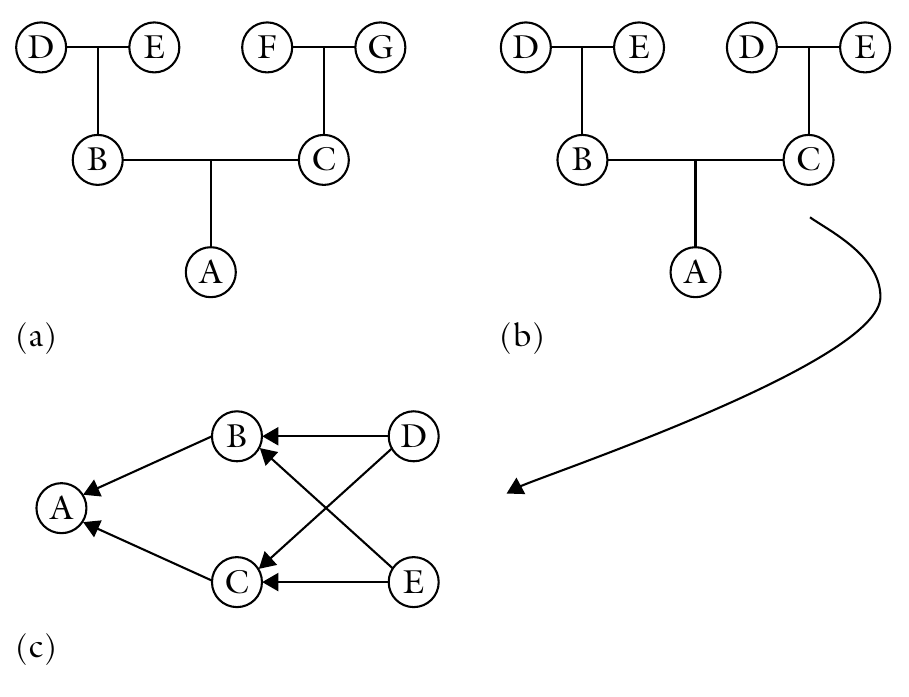
\includegraphics[width=0.45\linewidth]{../images/arrow_diagram} 

}

\caption{Pedigree diagrams can be drawn in the standard form (a, b) or converted to into an arrow diagram (c).}\label{fig:inbreeding-coefficient}
\end{figure}

\end{frame}

\begin{frame}{Genetic basis of heterosis}
\protect\hypertarget{genetic-basis-of-heterosis}{}

\begin{itemize}
\tightlist
\item
  To explain the genetic basis for why fitness lost on inbreeding tends
  to be restored upon crossing, two theories have been proposed.

  \begin{itemize}
  \tightlist
  \item
    Dominance theory: C.G. Davenport in 1908 and later by I.M. Lerner,
  \item
    Overdominance theory: Shull in 1908 and later by K. Mather and J.L.
    Jinks.
  \end{itemize}
\item
  A third theory, the mechanism of epistasis (non-allelic gene
  interactions), has also been proposed.
\end{itemize}

\end{frame}

\begin{frame}{Biometrics of heterosis}
\protect\hypertarget{biometrics-of-heterosis}{}

\begin{enumerate}
\tightlist
\item
  Better parent heterosis (Heterobeltiosis)
  \[Hybrid~vigour = \frac{F_1-Better~parent}{Better~parent}\]
\item
  Mid parent heterosis
  \[Hybrid~vigour = \frac{F_1-\frac{(P_1+P_2)}{2}}{\frac{(P_1+P_2)}{2}}\]
\item
  Commercial heterosis
  \[Hybrid~vigour = \frac{F_1-Commercial~Hybrid}{Commercial~Hybrid}\]
\end{enumerate}

\end{frame}

\begin{frame}{Types of hybrids}
\protect\hypertarget{types-of-hybrids}{}

\begin{itemize}
\tightlist
\item
  Commercial applications of hybrid breeding started with a cross of two
  inbred lines (a single cross - AxB) and later shifted to the more
  economic double cross, ({[}AxB{]}x{[}CxD{]}) and then back to a single
  cross.
\item
  Other parent combinations in hybrid development have been proposed,
  including the three-way cross ({[}AxB{]}xC) and modified versions of
  the single cross, in which closely related crosses showed that the
  single cross was superior in performance to the other two in terms of
  average yield.
\item
  However, it was noted also that the genotype x environment interaction
  (hybrid x environment) variability was more than twice that for the
  double crosses, while the mean variability for the three-way cross
  being intermediate.
\end{itemize}

\end{frame}

\begin{frame}{}
\protect\hypertarget{section-14}{}

\begin{itemize}
\tightlist
\item
  This indicated that the single crosses were more sensitive or
  responsive to environmental conditions than the other crosses.
\item
  Whereas high average yield is important to the producer, consistency
  in performance across years and locations (i.e., yield stability) is
  also important.
\item
  Double and three-way crosses have a more genetically divergent
  population for achieving buffering.
\item
  Today commercial hybrids are predominantly single cross, of best
  combining parental inbred lines.
\item
  For outline of mating scheme, See Lecture 7 on ``Hybridization
  techniques and its consequences'' (Course: Introductory plant
  breeding, \(4^{th}\) semester, BScAg).
\end{itemize}

\end{frame}

\hypertarget{numerical-problems}{%
\section{Numerical problems}\label{numerical-problems}}

\begin{frame}{Problem}
\protect\hypertarget{problem-1}{}

In blackgram, grain yield of parents (\(P_1\) and \(P_2\)) their \(F_1\)
and \(F_2\) progenies are given below:

\begin{table}[H]
\centering\begingroup\fontsize{6}{8}\selectfont

\begin{tabular}{rrrr}
\toprule
Parent 1 & Parent 2 & F1 hybrid & F2 progeny\\
\midrule
19 & 23 & 29 & 15\\
\bottomrule
\end{tabular}
\endgroup{}
\end{table}

Calculate average heterosis, heterobeltiosis and inbreeding depression.

\end{frame}

\begin{frame}{Solution}
\protect\hypertarget{solution-1}{}

\begin{equation}
\begin{aligned}
\text{Mid parent heterosis} &= \frac{F_1 - MP}{MP} \times 100\% \\
\text{Here, Value of } F_1 &= 29.38 \\
\text{Mean of parents (MP)} &= \frac{18.9+22.69}{2} = 20.81 \\
\text{Mid parent heterosis } &= \frac{29.38-20.81}{20.81} \times 100\% = 41.12\% \\
\text{Heterobeltiosis} &= \frac{F_1-BP}{BP} \times 100\% = \frac{29.38-22.69}{22.69} \times 100\% = 29.48\% \\
\text{Inbreeding depression} &= \frac{F_1-F_2}{F_1} \times 100\% = \frac{29.38-15.18}{15.18} \times 100\%= 48.33\%
\end{aligned}
\nonumber
\end{equation}

\end{frame}

\hypertarget{bibliography}{%
\section{Bibliography}\label{bibliography}}

\begin{frame}{References}
\protect\hypertarget{references}{}

\end{frame}




\end{document}
